\documentclass[a4paper,10pt,twocolumn]{article}

\usepackage[utf8]{inputenc}
\usepackage[T1]{fontenc}
\usepackage{lmodern}  % makes ligatures copy-pasteable

\usepackage[ngerman]{babel}

\usepackage{amsmath}
\usepackage{xcolor}

\usepackage{epsfig}
\usepackage{epstopdf}

\title{Simulation Rohrbruch Gasverteilnetz}
\author{}
\date{}

\begin{document}

\maketitle

\section{Problem-Domäne}

\begin{figure}[hbp]
\centering
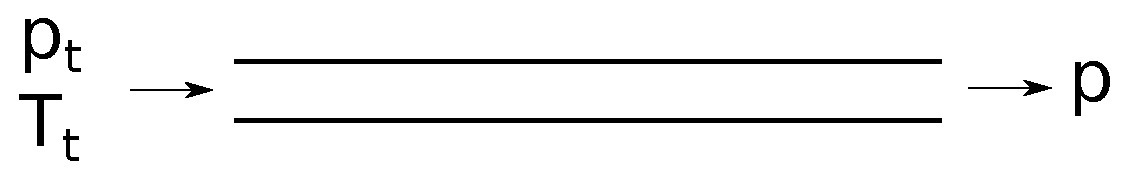
\includegraphics[width=0.9\hsize]{problem.eps}
\caption{Leitungssegment}
\end{figure}

\section{Modellierung}

\appendix

\section{Grundgleichungen}

\begin{equation}
M = 1 + \frac{\gamma-1}{\gamma} \mathit{Ma}^2
\end{equation}

\end{document}
